% siminos/atlas/cut.tex  pdflatex atlas
% $Author$ $Date$

\section{Dynamics and symmetries: a recap}
\label{s:cut}

\subsection{Group orbit}

    \ifdraft\color{blue}
%%%%%%%%%%%%%%%%%%%%%%%%%%%%%%%%%%%%%%%%%%%%%%%%%%%%%%%%%%%%%%%%%%%%%
\begin{figure}
   \centering
   %\includegraphics[width=0.45\textwidth]{???}
   \caption{\label{fig:tangents}
3 tangents: one $\vel(\ssp)$  and two group tangents
$\groupTan^{(1)}(\ssp)$, $\groupTan^{(2)}(\ssp)$.
}
\end{figure}
%%%%%%%%%%%%%%%%%%%%%%%%%%%%%%%%%%%%%%%%%%%%%%%%%%%%%%%%%%%%%%%%%%%%%

define
\begin{itemize}
  \item dynamical system $\{\pS,\map^t\}$ with symmetry \Group\
        vs reduced dynamics $\{\pSRed,\mapRed^t\}$
  \item \statesp\ vs tangent space, see \reffig{fig:tangents}
  \item time trajectory \flowRed{\zeit}{\ssp} vs group orbit
        $\pS_\ssp = \{\LieEl\,\ssp \mid \LieEl \in {\Group}\}$
  \item \template
  \item section {\PoincS} vs slice \pSRed
  \item strobing $\sim$ method of connections
  \item reduction vs projection
\end{itemize}
will explain later on
    \color{black}\fi

\subsection{\Statesp\ visualization}
\subsection{\CLe}
\subsection{Ring of Fire}
\subsection{Experimentalist description: a video 1D to 3D arrays of pixels}
\subsection{Theorist description: $\infty$-\dmn\ \statesp}
\subsection{Time orbit: point is a point, line is a line in all dimensions}
\label{sect:TimeOrb}

\subsection{Physical dimension: covariant Lyapunov vectors}

\section{Poincar\'e sections}
\label{s:cut}

In general there are two strategies for replacing a continuous-time flow
by iterated mappings; by cutting it by Poincar\'e sections, or by
\emph{strobing} it at a sequence of instants in time. While
`strobing' is what any numerical integrator does, by representing a
trajectory by a sequence of time-integration step separated points,
strobing is in general not a reduction of a flow, as the sequence of
strobed points still resides in the full \statesp\ $\pS$, of
dimensionality $d$.

In the {\em Poincar\'e section method} one records the coordinates of a
trajectory whenever the trajectory reaches a
triggering event. A Poincar\'e section (or, from now on,
just a `section') is {\em not} a projection onto a lower-dimensional space:
Rather, it is a local change of coordinates to a direction along the
flow, and the remaining coordinates (spanning the section) transverse to
it. No information about the flow is lost; the full
space trajectory can always be reconstructed by integration from the
nearest point in the section.

    \ifdraft\color{blue}
        There is always tension between mathematics - linear problem eigenmodes
        (Fourier for translations and rotations) and physics - the fact that
        nonlinear dynamics states are far away from such axes, as they
        always involve a number of such linear modes strongly entangled.
    \color{black}\fi

\subsection{Local chart}
After some experimentation and observations of chaos in a given
flow, one can identify a set of dynamically important unstable
{\recurrStr s}.

\subsection{R\"ossler {\poincBord}}

%%%%%%%%%%%%%%%%%%%%%%%%%%%%%%%%%%%%%%%%%%%%%%%%%%%%%%%%%%%%%%%%%%%%%
\begin{figure}
   \centering
   %\includegraphics[width=0.45
\begin{minipage}[b]{0.19\textwidth} %{0.39\textwidth}
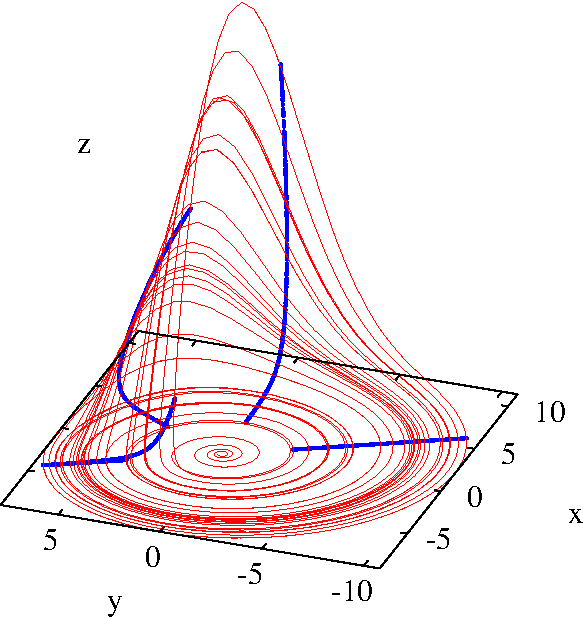
\includegraphics[width=1.15\textwidth,origin=c]
            {Rossler_PsectionB}
\\
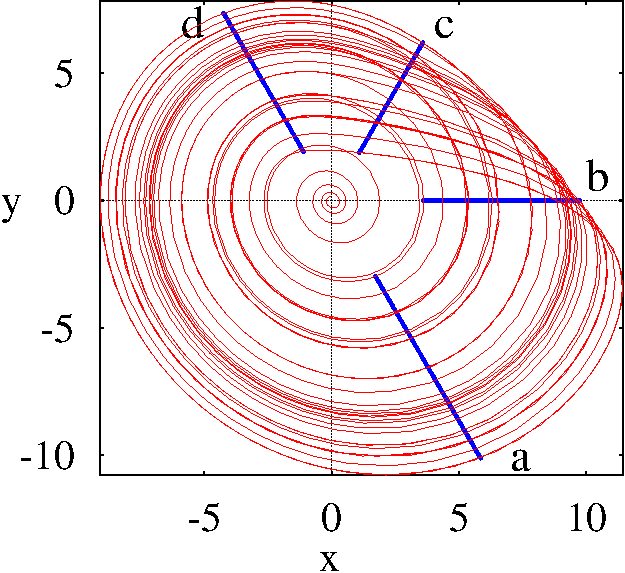
\includegraphics[width=0.80\textwidth,origin=c]
            {Rossler_PsectionA}
  \end{minipage}~~~~~%
  \begin{minipage}[b]{0.25\textwidth} %{0.50\textwidth}
    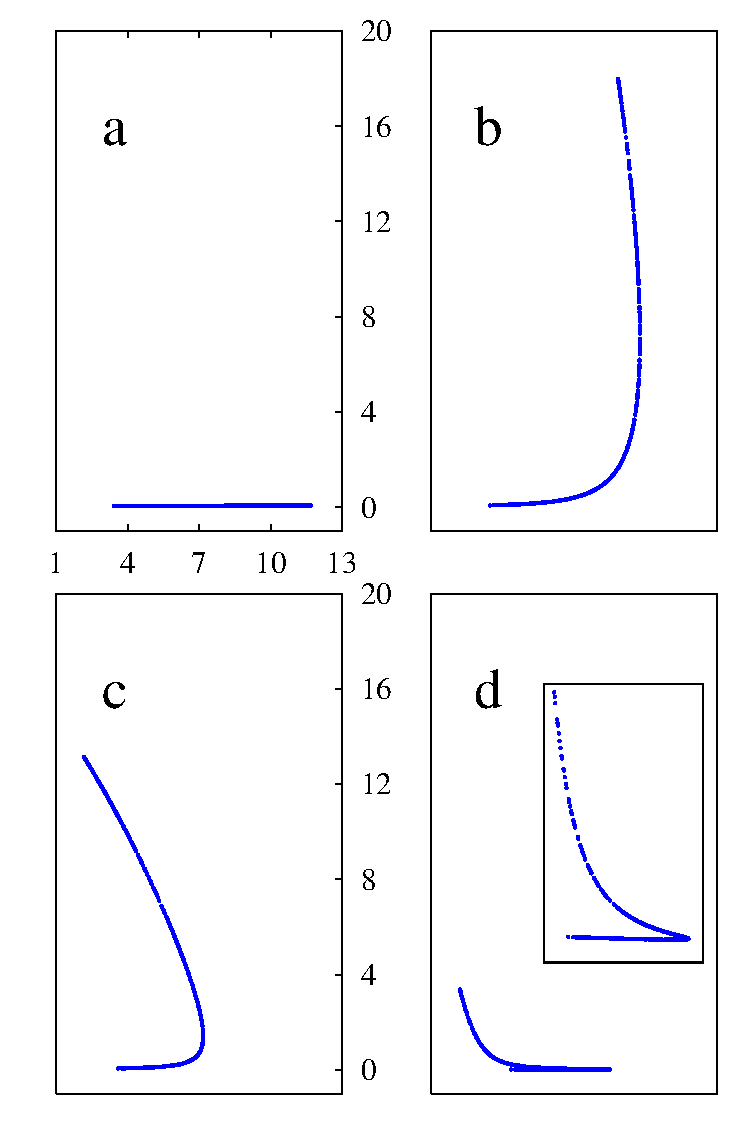
\includegraphics[width=1.00\textwidth]
            {Rossler_PsectionC}
  \end{minipage}
   \caption{\label{f:RosslSect}
      (Right:) a sequence of Poincar\'e sections of
      the R\"ossler strange attractor,
      defined by planes through the $z$~axis, oriented at angles
      (a) $-60^o$
      (b) $0^o$,
      (c) $60^o$,
      (d) $120^o$,
      in the $x$-$y$~plane.
      (Left:) side and $x$-$y$~plane view of a typical trajectory  with
      Poincar\'e sections superimposed.
      (R. Pa\v skauskas)
            }
\end{figure}
%%%%%%%%%%%%%%%%%%%%%%%%%%%%%%%%%%%%%%%%%%%%%%%%%%%%%%%%%%%%%%%%%%%%%

\subsection{R\"ossler two-chart atlas}
\subsection{R\"ossler unstable manifold curvilinear distance}
\subsection{R\"ossler return map}
\subsection{$N$-chart atlas, forward maps}
\subsection{Ring of Fire return map\rf{lanCvit07}}
